% table 1
\begin{table}[H]
    \centering
    \begin{tabular}{ | l | p{10cm} |}
    \hline
    \textbf{Use case name}    & Healthy Diet Analysis \\
    \hline
    \textbf{Actors}           & Customer, Database \\
    \hline
    \textbf{Description}      & Users learn their dietary habit and see what they ate, when they ate, how frequently they ate. Also, users learn which products contain which ingredient and sustenance values. User can set notifications.  \\
    \hline
    \textbf{Data}             & All past purchases, purchase times, frequencies, and amounts. \\
    \hline
    \textbf{Preconditions}    & At least one purchase from the user, food information is in database. \\
    \hline
    \textbf{Stimulus}         & Customer creates the request, and the request stimulates the system to respond. \\
    \hline
    \textbf{Basic flow}       & 1) User requests the analysis by using their interface. \newline 2) Database system takes this request from the interface and returns the purchase list. \newline 3) Healthy diet analysis method prepares the report and sends it to the user. \\
    \hline
    \textbf{Alternative flow} & 4) User decides that a product is harmful, the system notifies the user at the future purchases. \\
    \hline
    \textbf{Exception flow}   & If no past purchase data exist, or food database is missing, terminate the process. \\
    \hline
    \textbf{Post-conditions}  & User is notified in case of harmful products specified by the authorities. \\
    \hline
    \end{tabular}
    \label{tab:01healthy_diet_analysis}
    \caption{Healthy Diet Analysis Function}
\end{table}

\begin{figure}[H]
    \centering
    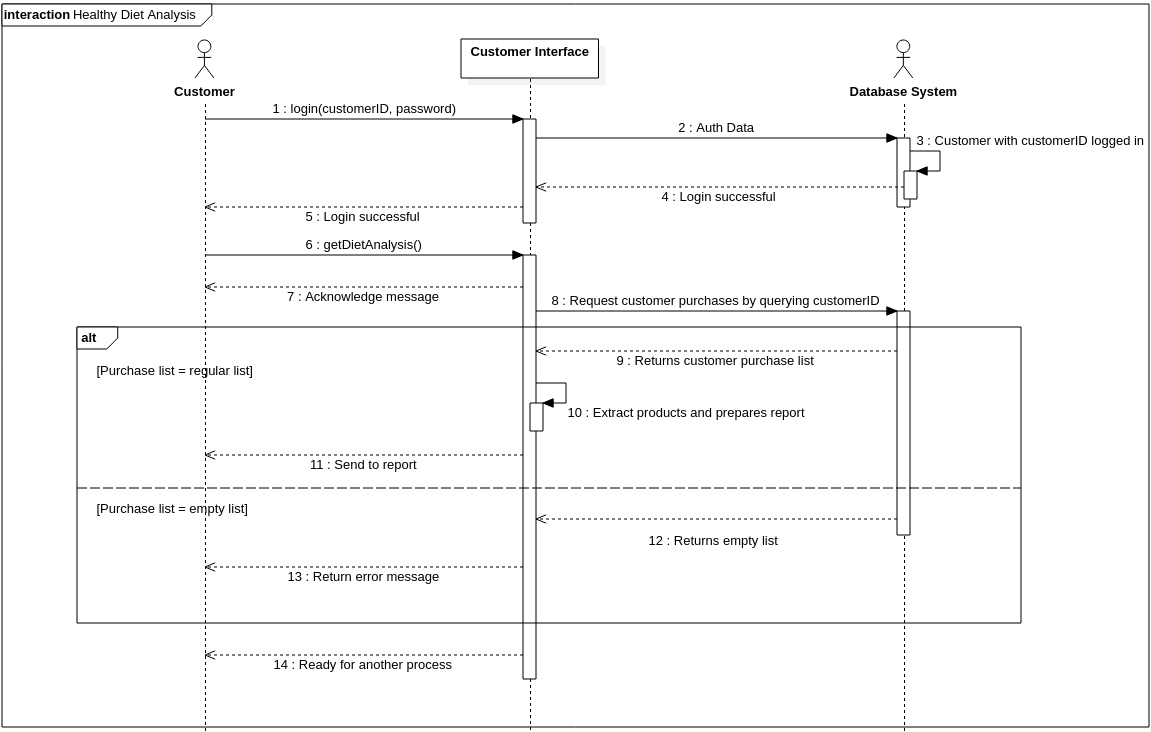
\includegraphics[width=0.99\linewidth]{content/specificRequirements/img/SequenceDiagramHealthyDietAnalysis.png}
    \caption{Sequence Diagram for "Healthy Diet Analysis" function}
    \label{fig:seq_diagram_healthy_diet}
\end{figure}

% table 2
\begin{table}[H]
    \centering
    \begin{tabular}{ | l | p{10cm} |}
    \hline
    \textbf{Use case name}    & Customer Support \\
    \hline
    \textbf{Actors}           & Store Staff, Customer \\
    \hline
    \textbf{Description}      & When customer needs any support, information request, system feature related information, or make any wrong transaction, store staff responds to the customer needs.  \\
    \hline
    \textbf{Data}             & Questions asked by the customer. \\
    \hline
    \textbf{Preconditions}    & When user is in trouble or in a situation where information is lacking. \\
    \hline
    \textbf{Stimulus}         & Any difficulty user experiences during the purchase which stimulates the store staff. \\
    \hline
    \textbf{Basic flow}       & 1) Customer request or asks about some stuff \newline 2) Store staff responds to the needs of the customer \\
    \hline
    \textbf{Alternative flow} & - \\
    \hline
    \textbf{Exception flow}   & - \\
    \hline
    \textbf{Post-conditions}  & - \\
    \hline
    \end{tabular}
    \caption{Customer Support Function}
    \label{tab:02customer_support}
\end{table}


% table 3
 \begin{table}[H]
     \centering
     \begin{tabular}{ | l | p{10cm} |}
     \hline
     \textbf{Use case name}    & Organize Products \\
     \hline
     \textbf{Actors}           & Store Staff \\
     \hline
     \textbf{Description}      & Store staff organizes the products in case of displacement of products through different shelves, or the products are broken because of some external force. Any physical damage to the objects that are not in the category of technical devices in the market are fixed by the store staff. \\
     \hline
     \textbf{Data}             & Broken object names and ids, displaced product names and ids. \\
     \hline
     \textbf{Preconditions}    & When some product is displaced because of any reason or some objects that are not counted as technical devices get damaged because of any external force.  \\
     \hline
     \textbf{Stimulus}         & Any broken, displaced, damaged object excites the staff. \\
     \hline
     \textbf{Basic flow}       & 1) An object gets some external impact. \newline 2) Store staff fixes the issue. \\
     \hline
     \textbf{Alternative flow} & 3) Store may choose to wait until the crowd in the market to decrease. \\
     \hline
     \textbf{Exception flow}   & 4) If the fix is not practical, then send the broken objects to external repair center. \\
     \hline
     \textbf{Post-conditions}  & Customers are notified in case of a possible danger because of the physical damage. \\
     \hline
     \end{tabular}
     \caption{Organize Products Function}
     \label{tab:03organize_products}
 \end{table}
 
 %TODO : above table, 3 and 4 will be 1 or 2.

% table 4
 \begin{table}[H]
     \centering
     \begin{tabular}{ | l | p{10cm} |}
     \hline
     \textbf{Use case name}    & Wrong Purchase Refund \\
     \hline
     \textbf{Actors}           & Customer, Bank \\
     \hline
     \textbf{Description}      & When a user decides to return the good, or there is a mistake in the decision making process resulting in wrong billing; the user can request a payback and get her/his refund from bank. \\
     \hline
     \textbf{Data}             & Purchase history, customer feedback and declaration, store product stock, transaction \\
     \hline
     \textbf{Preconditions}    & Wrongly done payment, incorrect item in checkout list of a user, damaged products cause the refund process.\\
     \hline
     \textbf{Stimulus}         & User applies for refund when he or she notices the extra payment or damaged product. \\
     \hline
     \textbf{Basic flow}       & 1) User requests for refund. \newline 2) The system is designed with the honor system(with an understanding that those looking to trick the system and steal things are in the minority). Thus, system accepts the refund request. \newline 3) Bank returns the extra money to the user back. \\
     \hline
     \textbf{Alternative flow} & 2) If the user makes frequent refund requests, system checks the user account and previous purchases in order to decide whether the user tries to trick the system or not.  \\
     \hline
     \textbf{Exception flow}   & 3) If user ID cannot be resolved, the refund request is ignored.  \\
     \hline
     \textbf{Post-conditions}  & User is notified about refund process by the bank. \\
     \hline
    \end{tabular}     \caption{Refund Function}
     \label{tab:04refund}
 \end{table}

% table 5
 \begin{table}[H]
     \centering
     \begin{tabular}{ | l | p{10cm} |}
     \hline
     \textbf{Use case name}    & Payment \\
     \hline
     \textbf{Actors}           & Customer, Bank \\
     \hline
     \textbf{Description}      & When a customer finishes shopping and exits from the store, total price of the products is drawn by the bank from the bank account of the user. This money will be deposited to the bank account of the Amazon Go store.  \\
     \hline
     \textbf{Data}             & Customer's latest shopping cart, product stock of the store \\
     \hline
     \textbf{Preconditions}    & User enters into the store by using mobile app QR code and purchases at least 1 product. \\
     \hline
     \textbf{Stimulus}         & When user leaves from store with products(a nonzero bill). \\
     \hline
     \textbf{Basic flow}       & 1) User exits from store with bought product/s. \newline 2) The system associates user with purchases. Also, it detects that user exited from the store. \newline 3) System automatically requests the total price of the products from the bank by giving customer credentials. \newline 4) Bank draws the total cost from customer's account and put that money into store's account.\\
     \hline
     \textbf{Alternative flow} & - \\
     \hline
     \textbf{Exception flow}   & 4) If user's account does not have sufficient money, bank uses credit for the user and put the money into the store's account. \\
     \hline
     \textbf{Post-conditions}  & Both user and store are notified by the bank about the latest transaction. \\
     \hline
     \end{tabular} \caption{Payment Function}
     \label{tab:05payment}
 \end{table}

 % table 6
 \begin{table}[H]
     \centering
     \begin{tabular}{ | l | p{10cm} |}
     \hline
     \textbf{Use case name}    & Customer Preferences \\
     \hline
     \textbf{Actors}           & Database, Customer \\
     \hline
     \textbf{Description}      & For each customer, system can predict next purchases of the customer since it keeps past purchases and their contents in the database system. \\
     \hline
     \textbf{Data}             & Past purchases of customers, purchase dates of customers, store \\
     \hline
     \textbf{Preconditions}    & At least 5 purchase has been completed by the customer. \\
     \hline
     \textbf{Stimulus}         & The system automatically starts to analyze past purchases when customer completed 5 purchases. \\
     \hline
     \textbf{Basic flow}       & 1) When a customer enters a store, get past purchase records and past purchase date data for all stores. Since past purchase information from the current store is more valuable, get the store id and separate past purchases information from the current store. 
     \newline 2) The system uses its own methods backed by machine learning to guess. \\
     \hline
     \textbf{Alternative flow} & - \\
     \hline
     \textbf{Exception flow}   & 1) If the database connection is lost due to a technical problem, system cannot take the necessary data. \\
     \hline
     \textbf{Post-conditions}  & System compares the actual bought products with its predictions for self learning/training mechanism. \\
     \hline
     \end{tabular} \caption{Customer Preference Function}
     \label{tab:customer_preference}
 \end{table}
 
 % TODO
 % alttakinin ismini degiselim cok fazla payment var banka baya ana rol ustleniyor gibi oldu
 % supply gibi bir sey yapalım
 % store staff dahil edelim
 
  % table 7
 \begin{table}[H]
     \centering
     \begin{tabular}{ | l | p{10cm} |}
     \hline
     \textbf{Use case name}    & Supply \\
     \hline
     \textbf{Actors}           & Supplier, Bank, Store Staff \\
     \hline
     \textbf{Description}      & Suppliers get their payment from the bank when they supply mass amount of products to the store. \\
     \hline
     \textbf{Data}             & Supplier credentials, total value of the supplied products, store \\
     \hline
     \textbf{Preconditions}    & Some of the products' stock values are decreased below a certain threshold(this threshold is defined for each product separately).  \\
     \hline
     \textbf{Stimulus}         & When a supplier brings requested products to one of the Amazon GO stores. \\
     \hline
     \textbf{Basic flow}       & 1) A supplier supplies products to a store at the same time store staff controls new products for damage/expire date. \newline 2) Supplier finishes his/her job in the store. \newline 3) Total bill is calculated by the system. \newline 4) System automatically start transaction in order to pay supplier. \\
     \hline
     \textbf{Alternative flow} & - \\
     \hline
     \textbf{Exception flow}   & 1) If new products do not have proper conditions, supply process is canceled. \\  
     \hline
     \textbf{Post-conditions}  & Database system is stimulated for stock renewing. \newline Store is notified for the money transaction by the bank. \\
     \hline
     \end{tabular} \caption{Mass Payment Function}
     \label{tab:07mass_payment}
 \end{table}

 % table 8
 \begin{table}[H]
     \centering
     \begin{tabular}{ | l | p{10cm} |}
     \hline
     \textbf{Use case name}    & Credentials \\
     \hline
     \textbf{Actors}           & Database, Customer \\
     \hline
     \textbf{Description}      & For each customer, system keeps his/her credentials like name, surname, contact information and bank account where further purchases can be drawn. \\
     \hline
     \textbf{Data}             & Customer \\
     \hline
     \textbf{Preconditions}    & A potential customer would like to use Amazon Go store since he/she wants to utilize store's innovation. \\
     \hline
     \textbf{Stimulus}         & A new customer downloads store's mobile application and starts typing his/her credentials. \\
     \hline
     \textbf{Basic flow}       & 1) Customer downloads the mobile app and launches it. \newline 2) In the welcome page, completes the tutorials/reads the guidelines.  \newline 3) In the registration page, he/she gives his/her name, surname, e-mail, address, phone number and credit card information. \newline 4) Customer is successfully registered to the system. \\
     \hline
     \textbf{Alternative flow} & 2) Some customers may skip this tutorials. \newline If a customer doesn't want to give credit card info at that moment, system lets the customer to register but it doesn't let the customer to shop until he or she give the credit card information. \\
     \hline
     \textbf{Exception flow}   & 3) If given credit card or phone number is not valid, the potential customer is not registered into the customer database. \newline 4) If any technical issue occurs in the process above, mobile app returns to the welcome page back and opens an error dialog. \\
     \hline
     \textbf{Post-conditions}  & Customer is informed for successfully registration. A welcome mail is sent to customer's mail address by the system automatically. \\
     \hline
     \end{tabular} \caption{Credentials Function}
     \label{tab:08credentials}
 \end{table}

 % table 9
 \begin{table}[H]
     \centering
     \begin{tabular}{ | l | p{10cm} |}
     \hline
     \textbf{Use case name}    & Analyze Logs \\
     \hline
     \textbf{Actors}           & Database, Technical Staff \\
     \hline
     \textbf{Description}      & Technical Staff views the system logs in order to maintain system.Logs will be saved in database system. \\
     \hline
     \textbf{Data}             & System Logs \\
     \hline
     \textbf{Preconditions}    & System is used by customers and logs are generated from different components of the system. Logs are sent and stored at database system. \\
     \hline
     \textbf{Stimulus}         & A specified system log review time for a technical personal comes. \\
     \hline
     \textbf{Basic flow}       & 1) Customer actions generate logs and these logs are saved on database. \newline 2) One of the technical staff personal logins and gets logs from database by using technical staff interface.  \newline 3) Technical staff personal reviews logs to learn about system usage. \\
     \hline
     \textbf{Alternative flow} & - \\
     \hline
     \textbf{Exception flow}   & -\\
     \hline
     \textbf{Post-conditions}  & System is maintained and improved by technical staff based on logs. \\
     \hline
     \end{tabular} \caption{Analyze Logs Function}
     \label{tab:09analyze_logs}
 \end{table}

\begin{figure}[H]
    \centering
    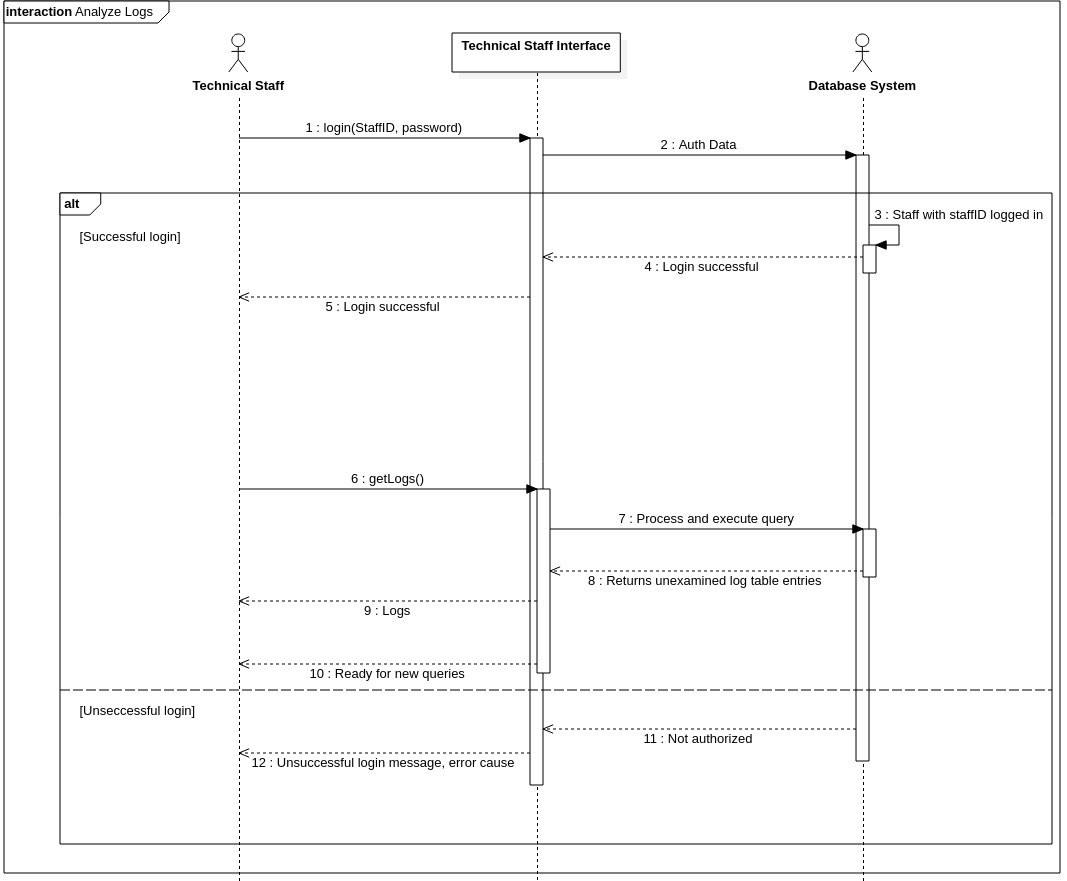
\includegraphics[width=0.99\linewidth]{content/specificRequirements/img/SequenceDiagramAnalyzeLogs.png}
    \caption{Sequence Diagram for "Analyze Logs" function}
    \label{fig:seq_diagram_analyze_logs}
\end{figure}
 
  % table 10
 \begin{table}[H]
     \centering
     \begin{tabular}{ | l | p{10cm} |}
     \hline
     \textbf{Use case name}    & Device Replacement \\
     \hline
     \textbf{Actors}           & Technical Staff \\
     \hline
     \textbf{Description}      & Technical Staff repairs/replaces a non-operating/broken sensors/electronic devices. These devices are detected by analyzing system logs.\\
     \hline
     \textbf{Data}             & System Logs \\
     \hline
     \textbf{Preconditions}    & System's electronic components logs their current situation into system. \\
     \hline
     \textbf{Stimulus}         & A device's logs are not in an expected fashion or no log can be taken from a dedicated device. \\
     \hline
     \textbf{Basic flow}       & 1) Technical staff detects that a device might not be working properly. \newline 2) One of the technical staff goes to the near place of it.  \newline 3) If the device is examined and is not working, technical staff removes it from the place. \newline 4) In order not to effect the effectiveness of the system, a new device is mounted at that place. \newline 5) Technical staff tries to repair non-operating component.\\
     \hline
     \textbf{Alternative flow} & 3) Device might be operating correctly but it doesn'l log due to a technical error. \newline 5) If non-operating device is broken, technical staff cannot repair it.  \\
     \hline
     \textbf{Exception flow}   & -\\
     \hline
     \textbf{Post-conditions}  & System is maintained and improved by technical staff. The replacing operation is saved into logs as well. \\
     \hline
     \end{tabular} \caption{Device Replacement Function}
     \label{tab:10device_replacement}
 \end{table}

% stock control

% table 11
 \begin{table}[H]
     \centering
     \begin{tabular}{ | l | p{10cm} |}
     \hline
     \textbf{Use case name}    & Stock Control \\
     \hline
     \textbf{Actors}           & Database \\
     \hline
     \textbf{Description}      & Database system checks the stock condition of the products regularly. If the remaining product number is less than a defined threshold (this threshold is unique for each product), it alerts the system.\\
     \hline
     \textbf{Data}             & Stock in database  \\
     \hline
     \textbf{Preconditions}    & A properly working database system is sufficient. \\
     \hline
     \textbf{Stimulus}         & A predefined time interval exceeds and database system automatically does the regular check. \\
     \hline
     \textbf{Basic flow}       & 1) Timer is set after each stock control. \newline 2) If timer interrupts, then database system does its regular check. \newline 3) If everything is fine, timer is set up again.\\
     \hline
     \textbf{Alternative flow} & 3) If one of the product stock level is less than predefined threshold, database system gives alert. \\
     \hline
     \textbf{Exception flow}   & -\\
     \hline
     \textbf{Post-conditions}  & The regular check and its results are saved into logs. \\
     \hline
     \end{tabular} \caption{Stock Control Function}
     \label{tab:11stock_controlt}
 \end{table}

% table 12
 \begin{table}[H]
     \centering
     \begin{tabular}{ | l | p{10cm} |}
     \hline
     \textbf{Use case name}    & Refund of Supply \\
     \hline
     \textbf{Actors}           & Supplier, Bank \\
     \hline
     \textbf{Description}      & When supplied products are not in a good condition(broken/expire date is not sufficient), store may request a refund from the supplier .\\
     \hline
     \textbf{Data}             & Supply  \\
     \hline
     \textbf{Preconditions}    & A group of product/s is supplied by the supplier. \\
     \hline
     \textbf{Stimulus}         & Store staff requests a refund bu using interface. \\
     \hline
     \textbf{Basic flow}       & 1) Supplier supplies requested products. \newline 2) Store staff checks the condition of products. \newline 3) If condition of some products are not good, refund process is initiated with the help of store staff interface. \newline 4) Total price of the supply is drawn from the supplier's bank account and put back to the store's account.\\
     \hline
     \textbf{Alternative flow} & 3) If products are in good condition, payment function is applied instead of refund function. \\
     \hline
     \textbf{Exception flow}   & -\\
     \hline
     \textbf{Post-conditions}  & Bank notifies both the supplier and store. \\
     \hline
     \end{tabular} \caption{Refund Function}
     \label{tab:12refund}
 \end{table}

% % table X
% \begin{table}[t]
%     \centering
%     \begin{tabular}{ | l | p{10cm} |}
%     \hline
%     \textbf{Use case name}    & Empty \\
%     \hline
%     \textbf{Actors}           & Empty \\
%     \hline
%     \textbf{Description}      & Empty \\
%     \hline
%     \textbf{Data}             & Empty \\
%     \hline
%     \textbf{Preconditions}    & Empty \\
%     \hline
%     \textbf{Stimulus}         & Empty \\
%     \hline
%     \textbf{Basic flow}       & Empty \\
%     \hline
%     \textbf{Alternative flow} & Empty \\
%     \hline
%     \textbf{Exception flow}   & Empty \\
%     \hline
%     \textbf{Post-conditions}  & Empty \\
%     \hline
%     \end{tabular}
%     \label{tab:01healthy_diet_analysis}
% \end{table}